\documentclass[11pt]{article}
\usepackage{longtable}
\usepackage{color}
\usepackage{tabu}
\usepackage{setspace}
\usepackage{pdflscape}
\usepackage{graphicx}
\usepackage {float}
%\usepackage{subfigure}
\usepackage{caption}
\usepackage{subcaption}
\usepackage{natbib}
\usepackage{fullpage}
\bibliographystyle{plain}
%\bibliographystyle{cbe}
\usepackage{algorithmic}
\usepackage[vlined,ruled]{algorithm2e}
\usepackage{amsmath}
\usepackage{amsfonts}
\usepackage{amssymb}
\usepackage[T1]{fontenc}
\usepackage{url}
 
\usepackage[dvipsnames]{xcolor}
\usepackage{color, soul}
\usepackage[colorlinks=true, linkcolor=blue, citecolor=DarkOrchid, urlcolor=TealBlue ]{hyperref}
%\usepackage[nottoc,numbib]{tocbibind}
\usepackage{tocloft}


\setlength\itemindent{0.25cm}

\newcommand{\phyg}{\texttt{PhyG} }
\newcommand{\BigO}[1]{\ensuremath{\mathcal{O}\left(\,#1\,\right)}\xspace}

\title{PhyG 0.3 Tutorials}

\author{Louise M. Crowley}
\makeindex
\begin{document}
\maketitle

\section{\phyg Tutorials}

These tutorials provide guidance for performing network analyses using the 
phylogenetic program \texttt{PhyG}. In addition to illustrating the vertical transfer 
of information between ancestor-descendant lineages, phylogenetic networks 
can convey information about reticulation events such as horizontal gene transfer, 
hybridization and introgression between lineages. There are two main types of 
networks---`softwired' and `hardwired'. When displayed, these networks main 
appear similar, however, they represent different interpretations of the meaning 
of phylogenetic edges.

A softwired network is a summary of a set of individual `display' trees or `tree-based 
networks', which have been generated by removing edges from the network.
In softwired networks, individual characters have single parents, as opposed 
to those in hardwired networks, where characters can have multiple parents 
\citep{KannanandWheeler2012}.

The user is advised to work through Tutorial 0.1 prior to attempting this tutorial, 
as this document provides instructions on obtaining and installing \texttt{PhyG}, 
as well as making and executing scripts. As in previous tutorials, each tutorial 
contains a \phyg script that includes detailed commentaries explaining the 
rationale behind each step of the analysis. The values of arguments herein have 
been chosen such that the analysis can complete within the timeframe of this 
session. Therefore, the values used here should not be taken to be optimal 
parameters. 

These tutorials use sample datasets that can also be downloaded from the 
\texttt{PhyG} \href{https://github.com/amnh/PhyGraph}{GitHub} website. Move 
these data files to a directory on your Desktop called \textbf{phygfiles}. The 
minimally required items to run the tutorial analyses are the \phyg application 
and sample data files. Running these analyses requires some familiarity with 
the \phyg command structure, to which a complete guide can be found 
\href{https://github.com/amnh/PhyGraph}{here}.

%-------------------------------------------------------------------------------------------------------
\subsection{Making a script and inspecting the data}
\label{subsec:networkscript}

In this tutorial, you will generate the initial script for a softwired network analysis 
and inspect the inputted data.

\begin{enumerate}

\item Open your text editor of choice and type the following:

	\begin{quote}	
	-\/-building networks for softwired tests using flu datasets\\
	set(seed:1634561640)\\
	set(outgroup:"1466\_H7N2\_Avian\_chicken\_pa\_1490921\_2002")\\
	set(graphtype:softwired)\\
	set(graphfactor:nopenalty)\\ 
	read(nucleotide:"flu*.fas*", tcm:(2,1))\\
	report("flu\_net1\_data.csv", data, overwrite)\\
	report("flu\_net1\_cr.csv", crossrefs, overwrite)
	\end{quote}

\item The script begins with a comment that describes the purpose of this 
analysis. Recall that comments are prepended with `-{}-' and can span multiple 
lines, provided each line begins with `-{}-'. \phyg will ignore any commented lines.\\

In the next four lines, we change the settings of \texttt{PhyG}. All \texttt{set}
commands are executed at the start of a run, irrespective of where they appear 
in the script. 

\item First, we \texttt{set} the seed for the random number generator to the 
integer value 1634561640. By setting this value, we are guaranteed to reproduce 
a given search trajectory each time the script is run.

\item Next, the outgroup for the analysis is \texttt{set} to 
\emph{1466\_H7N2\_Avian\_chicken\_pa\_1490921\_2002}. If the outgroup is not 
\texttt{set}, the default outgroup is the taxon whose name is lexically first after any 
renaming of taxa, and/or if taxa were specified by using the arguments \texttt{include}
or \texttt{exclude}. Only a single taxon can be set as the outgroup of the analysis. 
Recall that taxon names cannot have spaces, otherwise the names can be incorrectly 
interpreted by the program.

\item We next \texttt{set} the \texttt{graphtype} of this analysis. \phyg allows for 
the input, analysis of and output of a broader class of phylogenetic graphs. These
include trees, forests and both softwired and hardwired networks. The current choices 
are \texttt{tree} (the default), \texttt{hardwired} and \texttt{softwired}. We \texttt{set} 
the \texttt{graphtype} to \texttt{softwired}.

\item When conducting a network analysis, a penalty can be ascribed so that 
softwired phylogenetic networks can compete equally with phylogenetic trees on 
a parsimony optimality basis. A network penalty takes into account the change in 
cost as edges are added to the tree. Current choices include \texttt{nopenalty}, 
\texttt{w15} and \texttt{w23}. In general, \texttt{w23} is a more severe penalty than
\texttt{w15}. For the generation of an initial network for further analysis, we 
\texttt{set} the \texttt{graphfactor} to \texttt{nopenalty}. Note: assigning \texttt{nopenalty}
is fine for the generation of graphs for further refinement, however it is unlikely 
to be a reasonable penalty for `real' analyses.

\item Change to the directory where the downloaded data files are located by using the 
\texttt{cd} command, as in:
		
	\begin{quote}
	cd ~/Desktop/phygfiles
	\end{quote}

By typing \texttt{ls} you will see that this directory contains twelve files in fasta format.
A primary requirement of this type of analysis is to have a minimum of two blocks of 
data. The command \texttt{read} imports our data files. Rather than type in the name 
of each of these files in our script, we will use wildcards (*) to capture all these files: 
        
        \begin{quote}
	read(nucleotide:"flu*.fas*", tcm:(2,1)\\
	\end{quote}

Filenames must include the suffix (e.g. .fas, .fasta, .fastc, .ss, .tre). Note in this case, 
the wildcards capture files ending in .fasta and .fas. Failure to include these suffices 
will result in the error "File(s) not found in `read' command". The filename must match 
\textit{exactly}, including capitalization. We indicate that the files contain IUPAC 
\texttt{nucleotide} sequence data in fasta format.

\item Having read in our data, it is advisable to verify that the files were properly 
parsed. We \texttt{report} a \texttt{crossrefs} and \texttt{data} file, which allows us
to output information concerning the characters and terminals in our data files. 

\item Save this file with the name \textbf{flu\_net1.pg} in a directory \texttt{phygfiles} 
located on your Desktop.

\item Run the script by typing the following:

	\begin{quote}
  	phyg flu\_net1.pg
	\end{quote}

\item Examine the reported files \textbf{"flu\_net1\_data.csv"} and 
\textbf{"flu\_net1\_cr.csv"}. The \texttt{data} file summarizes information 
relating to the input data (number of terminals, number of input files, number of 
character blocks and the total number of characters). The \texttt{crossrefs} file
provides a comprehensive visual overview of the completeness of the data. Together
these files indicate that data has been input for nine terminal taxa, across 12 data 
blocks. The \texttt{crossrefs} file highlights that data is missing for three taxa.
\end{enumerate}

%-------------------------------------------------------------------------------------------------------
\subsection{Generating a network from trees}
\label{subsec:makinganetwork}

The first step in the analysis of networks is to generate one. Having imported and 
inspected our data, we are now ready to build the initial graphs. In this tutorial, you 
will learn how to generate a network from trees using \texttt{PhyG}. 

\begin{enumerate}

\item Modify the script to include \texttt{build(distance, rdwag, block, graph, eun, 
replicates:1000)}. By specifying \texttt{block}, \phyg performs independent builds 
for each ``block'' of data. If this option is not specified, the builds are performed 
combining all the data. This command causes a pairwise distance matrix to be 
calculated ($\BigO n^2$) that is subsequently used as a basis for distance tree 
construction. \texttt{distance} trees are constructed on the \texttt{block}s of data 
by performing random addition sequence distance Wagner builds, yielding multiple 
trees determined by the argument \texttt{replicates:n}. The resulting trees or 
\texttt{graph}s are reconciled using the \texttt{eun} argument, turning them into 
a network. \texttt{eun} reconciles block trees into a Edge-Union-Network 
\citep{MiyagiandWheeler2019, Wheeler2022}.

\item We want to examine the resulting trees. Trees are not reported as 
output in the terminal window and must be directed to a file. Modify the script 
to output tree files with \texttt{report("flu\_net1.tre", graphs, newick, overwrite)}
and \texttt{report("flu\_net1\_gv.tre", dotpdf, graphs, overwrite)}.

	\begin{quote}	
	-\/-building networks for softwired tests using flu datasets\\
	set(seed:1634561640)\\
	set(outgroup:"1466\_H7N2\_Avian\_chicken\_pa\_1490921\_2002")\\
	set(graphtype:softwired)\\
	set(graphfactor:nopenalty)\\ 
	read(nucleotide:"flu*.fas*", tcm:(2,1))\\
	build(distance, rdwag, block, graph, graph, eun, replicates:1000)\\
	report("flu\_net1\_data.csv", data, overwrite)\\
	report("flu\_net1\_cr.csv", crossrefs, overwrite)\\
	report("flu\_net1.tre", graphs, newick, overwrite)\\
	report("flu\_net1\_gv.tre", dotpdf, graphs, overwrite)
	\end{quote}
	
\item Run the script.

\item Let's examine the reported tree files. Because the file \textbf{"flu\_net1.tre"} 
represents a phylogenetic network (as opposed to tree), this file can not be viewed 
using tree viewing programs such as \textit{FigTree} or \textit{TreeView}. Using 
your preferred text editor, open this file. This looks like a standard newick tree file, 
in parenthetical notation, however, notice the addition of six \textbf{\#}'s, which 
represent reticulation events. The values associated with the taxon names and 
HTUs are the branch lengths. The cost of the tree(s) can be found in square 
brackets, at the end of each tree. In this analysis, \phyg returned a single network
 with a cost of 13930.

\item  The command \texttt{report("filename.tre", dotpdf, graphs, overwrite)} will 
produce a file that can be read in \textit{Adobe Illustrator}, \textit{Apple Preview} 
or any vectorial image editor program. Notice that two files were outputted from 
using this command. \phyg has output an eps (on OSX) or pdf (on linux) file that 
can be viewed in a vector graphics program and a dot file, which can be viewed 
(and modified) in \textit{Graphviz}. Note: in order to output pdf files the application 
\textit{dot} must be installed from the \href{https://graphviz.org/download/}{Graphviz} 
website. \textit{dot} is a graph description language and Graphviz an open-source 
graph visualization software. This program is well suited to representing graphs 
and networks. Open the reported file \textbf{"flu\_net1\_gv.tre.eps"} in your preferred
visualization program (Figure \ref{eps1}). The values associated with the taxon 
names and HTUs are the branch lengths. Examining this file, we can see three 
networks (leading into HTU14, HTU15 and HTU16).

\begin{figure}[H]
\centering
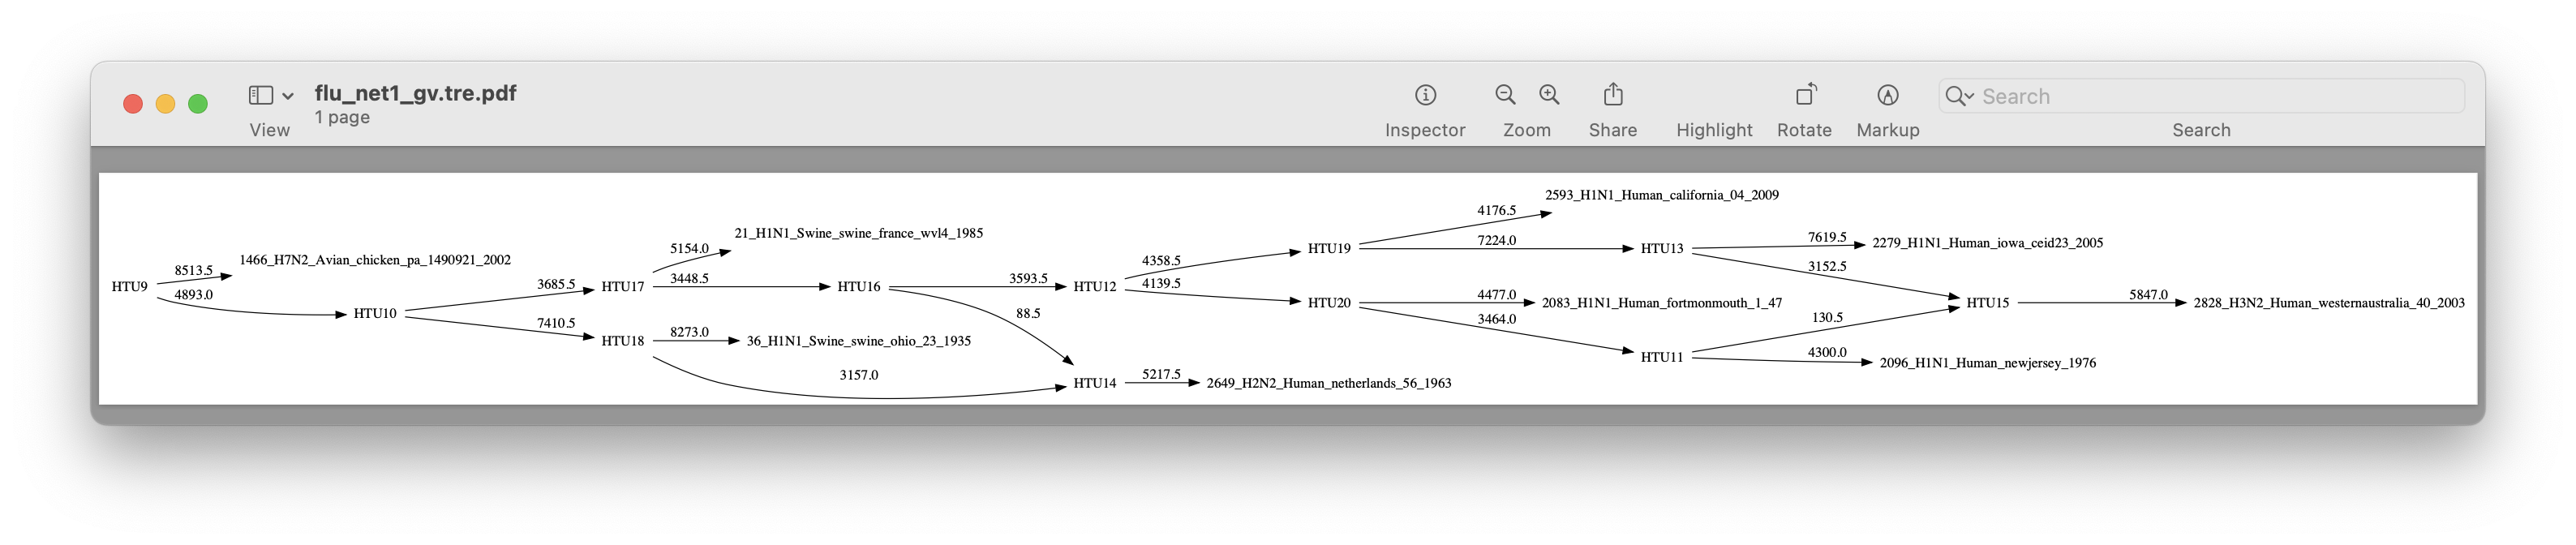
\includegraphics[width=\textwidth]{eps1.png}
\caption{\textbf{"flu\_net1\_gv.tre.eps"}.}
\label{eps1}
\end{figure}

\end{enumerate}
%-------------------------------------------------------------------------------------------------------
\subsection{Refining a network}
\label{subsec:refininganetwork}

Now that we have a network, we can perform some edit operations on the network
edges. In this tutorial we will learn how to add, delete, add-delete and move network
edges to the existing network graph.

\begin {enumerate}

\item Open your text editor of choice and type the following:

	\begin{quote}	
	-\/-Network refinements of networks using flu data sets\\
	set(seed:1634561640)\\
	set(outgroup:"1466\_H7N2\_Avian\_chicken\_pa\_1490921\_2002")\\
	set(graphtype:softwired)\\
	set(graphfactor:w23)\\ 
	read(nucleotide:"flu*.fas*", tcm:(2,1))\\
	read(newick:"flu\_net1.tre")\\
	refine(netadd, atrandom, steepest)\\
	report("flu\_net2.tre", graphs, newick, overwrite)\\
	report("flu\_net2\_gv.tre", dotpdf, graphs, overwrite)
	\end{quote}

\item The script begins with a comment that describes the purpose of this 
analysis.

\item The next three lines of this script are identical to that of \textbf{flu\_net1.pg}, 
so we will not comment about them here. 

\item Unlike the previous script, here we \texttt{set} the \texttt{graphfactor} to 
\texttt{w23}. This penalty does not involve the calculation of the Maximum 
Parsimony display tree, therefore it has a lower time complexity to calculate
the penalty.

\item Save this file with the name \textbf{flu\_net2.pg} in the same directory as the 
data files and previously reported trees.

\item

\item

\item



\end{enumerate}

%-------------------------------------------------------------------------------------------------------


%\printindex
\bibliography{/Users/louise/DropboxAMNH/big-refs-3.bib}
\end{document}
